
\section{Properties of \acs{BSCO}}
\label{Sec:Intro:PropertiesBSCO}

The unit cell of the high--$T_c$, doped cuprate \acf{BSCO} is illustrated in figure~\ref{Fig:Intro:BSCOUnitCell}. It is made up of layers as follows from the top; a BiO layer, then a SrO layer, then a CuO layer common to all cuprates, then two BiO layers, a SrO layer, a CuO, SrO and a BiO layer. Variants of \acs{BSCO} include \ac{BSCO2212} and \ac{BSCO2213} which feature one and two extra CuO layers respectively. Most closely related in terms of structure is \acs{TL2201} which features Tl and Ba in place of Bi and Sr respectively. \ac{BSCO} is orthorhombic with $a=\unit{5.362(3)}{\angstrom}$, $b=\unit{5.374(1)}{\angstrom}$ and $c=\unit{24.622(6)}{\angstrom}$~\cite{Torardi1988a}, \ac{TL2201} on the other hand has $a=\unit{5.4580(3)}{\angstrom}$, $b=\unit{5.4848(5)}{\angstrom}$ and $c=\unit{23.2014(5)}{\angstrom}$~\cite{Peets2007}.
\begin{figure}[htbp]
    \begin{center}
        \includegraphics[scale=1.1]{Chapter-Introduction/Figures/BSCOUnitCell/BSCOUnitCell}
        \caption{Unit cell of \acs{BSCO} demonstrating the layers. \ac{TL2201} is similar but with La for Bi and Ba for Sr. Note that Pb doping occurs away from the CuO planes.}
        \label{Fig:Intro:BSCOUnitCell}
    \end{center}
\end{figure}
Undoped \ac{BSCO} has an excess of holes and lies slightly to the underdoped side of the phase diagram. By substituting in La for Sr, the amount of holes is reduced allowing access to a range of slightly overdoped to underdoped. However, since the substitution takes place adjacent to the CuO planes where all the interesting electronic behaviour happens, La doping introduces a lot of disorder into the system. Pb is also substituted for Bi which increases the number of holes allowing the more overdoped region to be accessed. Since Pb substitutes into the BiO layer which is far from the CuO plane, less disorder is introduced. Sometimes Pb is introduced alongside La even when a more underdoped state is desired to avoid forming structures in the BiO planes which affect \ac{ARPES} measurements~\cite{Kondo2007}. Furthermore, annealing in oxygen decreases the number of carriers depending on how much additional oxygen is absorbed allowing for even more fine grained tuning of the doping. By adjusting these parameters a very wide range of doping values can be accessed in \ac{BSCO} which makes it appealing for study.

\begin{figure}[htbp]
    \begin{center}
        \includegraphics[scale=1.0]{Chapter-Introduction/Figures/VanHoveBSCOLSCO/VanHoveBSCOLSCO}
        \caption{Band dispersions at the Fermi energy for various dopings. Left panel shows \ac{BSCO}, right panel shows \ac{LSCO}. Note the saddle points at $(\pi, 0)$ which cause the van-Hove singularity at $p\approx 0.18$ for \ac{LSCO} and at $p \geq 0.2$ for \ac{BSCO}. Adapted from ref.~\cite{Hashimoto2008}.}
        \label{Fig:Intro:VanHoveBSCOLSCO}
    \end{center}
\end{figure}

\subsection{Fermiology of \ac{BSCO}}

There is a crossover in overdoped cuprates between a large hole-like Fermi surface to an electron-like Fermi surface that leads to a saddle point in the \ac{DOS} and consequently a van Hove singularity as shown in figure~\ref{Fig:Intro:VanHoveBSCOLSCO}, which is adapted from \ac{ARPES} results from ref.~\cite{Hashimoto2008}. This occurs in \ac{LSCO} at around $p\approx0.18$ which is approximately critical doping and may lead one to believe that the critical behaviour is related to the proximity of the van Hove singularity. However the same crossover does not happen at the same doping in \ac{BSCO}, rather it appear to occur at $p \geq 0.2$, relatively far from the critical value of $p \approx 0.16$. For this reason \ac{BSCO} is an attractive material to study to determine more about the relationship (or lack thereof) between the critical behaviour and the van Hove singularity.

% Finally \ac{BSCO} has a relatively low maximum $T_c$, being around
% \unit{36}{\kelvin} at best. Because $T_c$ is so low, this makes
% \ac{BSCO} ideal for normal state study since less field will be
% required to suppress $T_c$ at lower temperatures and there should be a narrower fluctuation region.

\subsection{Determining the doping}
    \label{Sec:Intro:DeterminingDoping}

The precise determination of doping from a chemical standpoint is tricky. For \ac{LSCO} --- assuming pure ionic donation --- substituting more Sr for La simply adds one more hole per extra Sr atom per unit cell. However for \ac{Y123} and \ac{Y124} for example, there exist CuO chains (oxygen deficient CuO layers) which absorb some of the doped charge, in other cuprates the heavy metal atom has a mixed valency meaning that the substitution relation is not so straightforward. Various techniques are employed to determine the doping level but as a rule some a priori knowledge of composition is required.

Typically \ac{BSCO} doping is determined by matching the $T_c$ normalised to the maximum $T_c$ to a `universal' parabola determined by Presland \etal~\cite{Presland1991} or more recently by comparing Hall data to the well defined doping of \ac{LSCO}~\cite{Ando2000}. However there are concerns as to whether it is appropriate to compare \ac{BSCO} to \ac{LSCO} when it comes to the Hall data in the overdoped side of phase diagram due to the proximity of the van-Hove singularity.

However, recently the doping of \ac{TL2201} in overdoped samples was well characterised by \ac{dHvA} measurements of the Fermi surface~\cite{Rourke2010b} which through the Luttinger sum rule, based on the size of the Fermi surface volume, assigned higher dopings to the \ac{TL2201} samples than samples of \ac{LSCO} of comparable $T_c$. Given that structurally, \ac{BSCO} is much more similar to \ac{TL2201} than \ac{LSCO} and \ac{TL2201} is also not in immediate proximity to the van-Hove singularity, it may be preferable to compare the $R_H$ values in \ac{BSCO} to \ac{TL2201} using a method similar to that used by Ando \etal

\subsection{Motivation}

Original motivation for the high field transport measurements on \ac{BSCO} was to recreate the magnetoresistance measurements performed on \ac{LSCO} on a different material which is not so close to a van-Hove singularity to elucidate whether the highly unusual `foot' shape for the $T$-linear region is specific to \ac{LSCO} or more general to the cuprates. Moreover \ac{BSCO} allows for wider doping into the underdoped region --- resistivity in \ac{LSCO} diverges on the underdoped side at low temperatures --- and so will allow us to observe how the progression continues.  \ac{BSCO} also demonstrates transport behaviours which are consistent with other high-$T_c$ cuprate materials, for example, from resistance measurements it demonstrates a similar maximum in the underdoped $d\rho_{ab}/dT$ curve as underdoped YBCO~\cite{Ando1999} and on the overdoped side, \ac{BSCO} demonstrates a monotonic upward trend in $d\rho_{ab}/dT$ with increasing temperature similar to what has been observed in \ac{TL2201} and \ac{LSCO}~\cite{Ando1999}.

During the course of the investigations however, it became apparent that even with field strengths of up to \unit{60}{\tesla} in pulsed fields, the upper critical field, $H_{\textrm{c2}}$ of many of the samples at key temperatures could not be reached despite their relatively low $T_c$ which would imply narrower fluctuation regimes. However, field strengths were generally strong enough to recover $B$-Linear behaviour in the Hall component.

By examining the temperature dependence of Hall data down to \unit{1.4}{\kelvin} in \ac{BSCO} and applying a model based on anisotropic scattering and the Ong construction we can determine whether it is necessary to invoke the complex Fermi surface re-construction scenario described by LeBoeuf \etal to describe the behaviour of $R_H$.

Previous Hall measurements have been performed on \ac{BSCO} by Ando \etal~\cite{Ando1999, Ando2000} which are shown for comparison in the results section~\cite{Ando1999}. However these results do not go to low temperatures, being restricted by the onset of superconductivity. Our own results used high field measurements at \ac{LNCMI} and \ac{HFML} to suppress superconductivity and examine the low temperature regions in detail. Moreover our samples are focused on the overdoped region which complements the underdoped data set presented in the Ando and Balkirev papers~\cite{Balakirev2003}.

Furthermore, we can study the Hall effect to investigate the doping determination according to \ac{TL2201} described previously. We compare the data with results from \ac{ARPES} by our collaborators on the samples from the same batch which determine the doping directly, rather than inference through comparison to \ac{TL2201}, by measuring the size of the Fermi surface within the \ac{BZ}~\cite{Kondo2004}. The investigations described in this section are presented in chapter~\ref{Sec:HallBSCO}.

% Performing measurements which would shed light onto which of the scenarios shown in fig~\ref{Fig:Intro:PGScenario} is most likely to be correct formed the original motivation for the investigation of \ac{BSCO} through transport measurements. 

